\subsection{ Fiducial cut tent function}\label{sec:p_tent_function}

\begin{verbatim}

double tent(double *X, double *par) {
    double x = X[0];

    double p0 = par[0];
    double p1 = par[1];
    double p2 = par[2];
    double p3 = par[3];
    double p4 = par[4];
    double a  = par[5];

    // parabola parameters
    // y = ax2 + bx + c
    // a = par[5]
    // with two constrains given by the two points at x,y = (p1, p4), (p2, p4):
    double b = -a * (p1 * p1 - p2 * p2) / (p1 - p2);
    double c = p4 - a * p1 * p1 - b * p1;

    if (x < p1 - p0) return 0;                                      // no signal
    if (x >= p1 - p0 && x < p1) return (p4 / p0) * (x - p1 + p0);   // steep rise
    if (x >= p1 && x < p2) return a * x * x + b * x + c;            // parabola
    if (x >= p2 && x < p2 + p3) return (p4 / p3) * (-x + p2 + p3);  // steep descend
    if (x >= p2 + p3) return 0;                                     // no signal

    return 0;
}

\end{verbatim}

\vspace{-0.5cm}
\begin{figure}[h]
 \begin{center}
 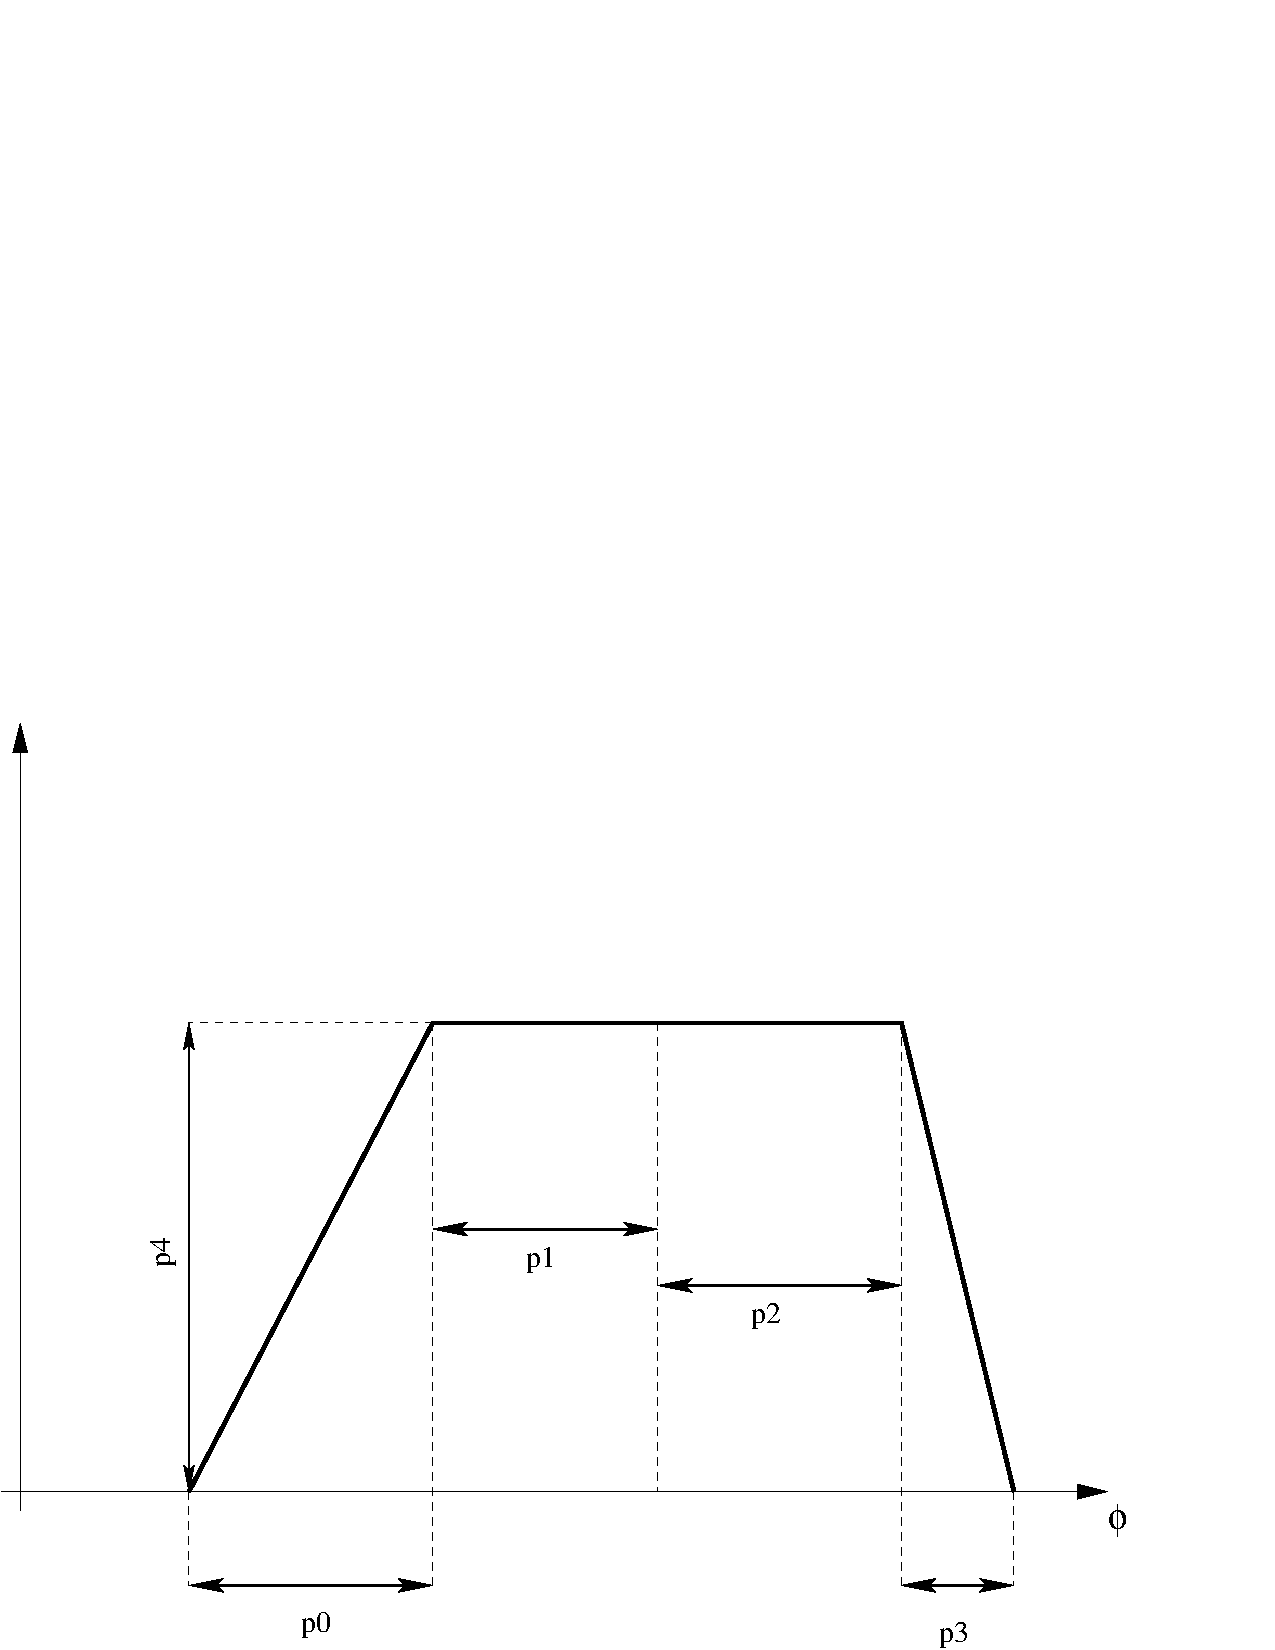
\includegraphics[width = 10cm, bb=-40 20 580 440]{img/traped}
  \caption[The trapezoid function used for the $\phi$ fit]
          { The trapezoid function used for the $\phi$ fit. The parameters $p_1$ and $p_2$ determine
                     the fiducial cut lower and upper limits.  }
 \end{center}
\end{figure}
The trapezoid fit gives the parameters $p_1$ and $p_2$ described above for each $\theta$ considered
in each momentum bin.